\chapter{NetLogo e DesignPattern}
In questo capitolo si fornisce una descrizione dell'ambiente NetLogo e dei Design Patterns che questo progetto usa al fine di una migliore comprensione e chiarezza dei concetti esposti nel Capitolo \ref{cap:sviluppo-progetto}.
\section {NetLogo} 
\label{sec:netlogo}
NetLogo \nocite{wilensky-tisue} \cite{netlogo} è un linguaggio di programmazione e un ambiente di modellazione di sistemi complessi. Adatto per la simulazione e lo studio di fenomeni naturali e sociali che si evolvono nel tempo.\\
Gli utenti possono dare istruzioni a migliaia di agenti che operano in modo concorrenziale. Questi comandi possono essere dati in modo individuale o collettivo, permettendo quindi lo studio dei comportamenti su più livelli, come quello microscopico dei behaviors individuali o quello macroscopico delle loro interazioni con gli altri.\\
NetLogo è usato per costruire una infinita varietà di simulazioni. I suoi turtles sono stati trasformati in molecole, lupi, clienti, commercianti, api, uccelli, batteri, macchine, magneti, pianeti, formiche e molto altro. Le sue patches allo stesso modo sono state usate come alberi, muri, corsi d'acqua, cellule tumorali, cellule vegetali e altro ancora. Turtles e patches possono essere usate per studiare astrazioni matematiche, ma anche per fare arte o giocare.\\
Tra i temi studiati con questo strumento ci sono automi cellulari, algoritmi genetici, evoluzione, ottimizzazione e individuazione di percorsi, dinamiche della popolazione e società artificiali.\\
Tutti questi modelli condividono il topic centrale perseguito da questo strumento che sono i sistemi complessi e i comportamenti emergenti.\\
Il più grande miglioramento apportato a partire dalla versione 2.0 in poi riguarda la grafica. In particolare i turtles possono essere di qualsiasi forma e dimensione e soprattutto possono essere posizionati in qualsiasi punto dello spazio. La loro grafica è di tipo vettoriale in modo da non avere perdita di qualità dell'immagine a qualsiasi scala si visualizzi il modello.\\
Uno dei principali obbiettivi di NetLogo è quello di essere scientificamente riproducibile, quindi i suoi modelli operano in modo deterministico. Inoltre le librerie matematiche Java platform-indipendent su cui si basa aiutano a dare consistenza e a rendere NetLogo indipendente dalla macchina su cui viene eseguito.\\

\subsection{Storia}
Nasce a scopo educativo e di ricerca, dalla fusione di \textbf{Logo} \cite{logo} e \textbf{StarLisp} \cite{starlisp}. Dal primo eredita il principio \textit{”low threshold , no ceiling”}, ovvero bassa soglia di conoscenza per il suo utilizzo, rendendolo accessibile a utenti inesperti nella programmazione, ma allo stesso tempo completa programmabilità, rendendolo quindi anche uno strumento utile per la ricerca.\\
Da Logo viene ereditato anche il concetto fondamentale di \textit{turtle}, con la differenza che Logo permetteva il controllo di un unico agente, mentre un modello NetLogo può averne migliaia. Da StarLisp, invece, NetLogo eredita i molteplici agenti e la loro \textit{concurrency}.\\
Il design di NetLogo si basa sulla precedente esperienza dei suoi creatori con StarLogoT \cite{starlogot}, di cui sono stati rielaborati quasi interamente sia l'interfaccia che il linguaggio, aggiungendo soprattutto funzionalità destinate a utenti nel campo della ricerca.

\subsection{Linguaggio}
Come linguaggio NetLogo si evolve da Logo al quale aggiunge il concetto di agenti e di concurrency. In generale Logo è molto conoscuto per il concetto di \textbf{\texttt{turtle}} che ha introdotto. NetLogo generalizza questo permettendo il controllo di centinaia o migliaia di turtles che si muovono e interagiscono tra di loro.\\
Il mondo in cui i turtles si muovono è suddiviso in \textbf{\texttt{patches}} anche esse interamente programmabili e identificabili attraverso coordinate spaziali.\\
Turtles e patches vengono chiamate collettivamente \textbf{\texttt{agents}}. Tutti gli agenti possono interagire tra di loro e eseguire istruzioni in modo concorrenziale.\\
NetLogo include inoltre un terzo tipo di agente, l'\textbf{\texttt{observer}} il quale è unico. In generale l'observer è quello che impartisce ordini agli agenti.\\
Possono essere definite diverse “razze” (\textbf{\texttt{breeds}}) di turtles, ciascuna con variabili proprie. In questo modo è possibile definire comportamenti caratteristici e distinti per ogni breed definita.\\
Una peculiarità che contraddistingue NetLogo dai suoi predecessori sono gli “\textit{agentsets}”, ovvero insiemi di agenti componibili anche al volo nel momento del bisogno. Questa caratteristica ha aumentato notevolmente la capacità espressiva del linguaggio in quanto permette di selezionare insiemi di agenti, anche eterogenei, che soddisfano condizioni arbitrarie a cui impartire istruzioni specifiche.\\
Si possono dichiarare tre tipi diversi di variabili: globali, locali e proprietarie. Le variabili globali possono essere modificate da qualsiasi parte del codice e vengono dichiarate fuori da qualsiasi procedura. Le variabili locali, invece, hanno visibilità limitata alla procedura in cui vengono dichiarate. Le variabili proprietarie, infine, sono associate esclusivamente alle  turtles o patches oppure a una specifica breed di esse.\\
Le procedure sono definite tutte in un unico file insieme alle variabili e sono destinate all'esecuzione da parte di specifici agenti oppure dell'observer stesso. Si possono definire procedure reporter o subroutine, dette anche command. Entrambe possono ricevere parametri in ingresso, la loro differenza sta nel fatto che i reporters, al contrario delle subroutine, restituiscono un valore in uscita. Quindi mentre le prime vengono usate per calcolare determinati valori e reperire specifiche informazioni, le seconde vengono usate per impartire istruzioni ad agenti e produrre effetti su variabili e altri agenti.\\
Concludendo, il linguaggio presenta tutti i costrutti standard come procedure, loop, liste, integrati con particolari costrutti per il supporto alla modellazione multi-agente.

\section{Pattern Builder}
\label{sec:builder}
Lo scopo di questo pattern è quello di separare la costruzione di un oggetto complesso dalla sua rappresentazione, in modo che il medesimo processo possa essere usato per creare rappresentazioni diverse.
\begin{figure}[htbp]
\centering
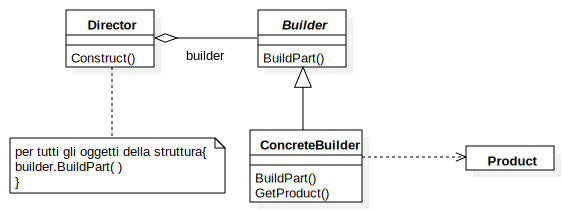
\includegraphics[width=\textwidth,height=\textheight,keepaspectratio]{images/builder-design-pattern.pdf}
\caption{Class diagram di un generico Builder}
\label{fig:builder-design-pattern}
\end{figure}
\subsection{Applicabilità}
Il pattern Builder è solitamente usato nei seguenti casi:
\begin{itemize}
\item l'algoritmo per la creazione di un oggetto deve rimanere separato dalle parti che lo costituiscono e dal modo in cui esse sono composte;
\item il processo di costruzione deve rendere possibili diverse rappresentazioni dell'oggetto a cui è associato.
\end{itemize}
\subsection{Partecipanti}
Il Builder coinvolge le seguenti classi:
\begin{itemize}
\item \textbf{Builder} mette a disposizione un interfaccia per la costruzione delle parti dell'oggetto '\textit{Product}'
\item \textbf{ConcreteBuilder} 
	\begin{itemize}
	\item Costruisce le parti dell'oggetto e le assembla secondo una specifica rappresentazione.
	\item Definisce e tiene traccia delle varie rappresentazioni create.
	\item Espone un metodo per ottenere il Product creato.
	\end{itemize}
\item \textbf{Director} sfrutta l'interfaccia del Builder per costruire il Product.
\item \textbf{Product} è l'oggetto complesso che viene costruito. ConcreteBuilder provvede a costruire le sue parti e definisce il processo con cui vengono assemblate. 
\end{itemize}
\subsection{Collaborazioni}
Il tipico funzionamento del Builder comporta le seguenti cooperazioni:
\begin{itemize}
\item Il Client mette in vita il Director e lo configura con il Builder corrispondente alla rappresentazione che desidera costruire.
\item Director manda una richiesta ogni volta che una parte del Product deve essere costruita.
\item Builder riceve le richieste del Director, costruisce e compone le parti del Product.
\item Il Client recupera dal Builder il Product costruito.
\end{itemize}
\begin{figure}[htbp]
\centering
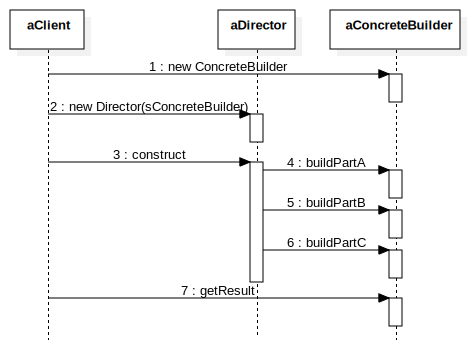
\includegraphics[width=\textwidth,height=\textheight,keepaspectratio]{images/builder-pattern-sequence.pdf}
\caption{Sequence Diagram di un generico Builder}
\label{fig:builder-pattern-sequence}
\end{figure} 


\subsection{Conseguenze}
L'introduzione del Builder in un progetto software produce le seguenti conseguenze:
\begin{enumerate}
\item Consente di variare la rappresentazione interna di un prodotto. Il Builder infatti, grazie alla sua interfaccia, nasconde la struttura interna dell'oggetto che costruisce, quindi per modificarla basta usare una diversa implementazione di questa interfaccia.
\item Migliora la modularizzazione incapsulando il codice necessario alla costruzione dei prodotti. In questo modo i client non hanno bisogno di conoscere la struttura interna dei prodotti. Inoltre Director diversi possono costruire varianti del prodotto con le stesse tipologie di parti interne.
\item Fornisce un controllo sul processo di costruzione molto ravvicinato. Al contrario di altri pattern creazionali che restituiscono il prodotto in un 'colpo' solo, questo segue il processo passo per passo rendendolo molto più controllato e sicuro.
\end{enumerate}

\section{Pattern Visitor}
\label{sec:visitor}
Visitor è uno pattern molto utile che consente di aggiungere nuove funzionalità alle parti di un oggetto composito senza modificare gli oggetti stessi.
\begin{figure}[htbp]
\centering
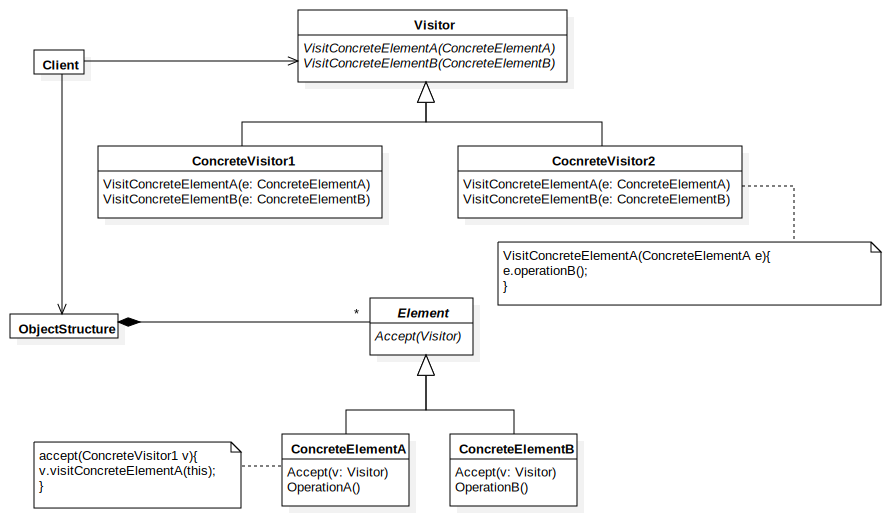
\includegraphics[width=\textwidth,height=\textheight,keepaspectratio]{images/visitor-design-pattern.pdf}
\caption{Class Diagram di un generico Visitor}
\label{fig:visitor-design-pattern}
\end{figure}

\subsection{Applicabilità}
L'utilizzo del pattern Visitor è consigliato nelle seguenti situazioni:
\begin{itemize}
\item Quando si devono eseguire operazioni diversificati in base alla classe concreta degli oggetti che compongono una struttura, ma questi presentano interfacce diverse.
\item Quando devono essere aggiunte operazioni su alcuni oggetti evitando di inquinare le loro interfacce.
\item Quando si ha un frequente bisogno di aggiungere funzionalità a classi che invece cambiano di rado. Infatti nel caso in cui queste classi dovessero cambiare, si dovrebbero modificare e aggiornare tutti i Visitor ad esse associati.
\end{itemize}

\subsection{Partecipanti}
Nell'implementazione di questo pattern vengono coinvolte le seguenti classi:
\begin{itemize}
\item \textbf{Visitor} definisce un metodo per ogni ConcreteElement, in modo tale da essere in grado di capire il tipo concreto dell'oggetto che ha chiamato il metodo.
\item \textbf{ConcreteVisitor} implementa tutti i metodi definiti da Visitor. Fornisce inoltre un contesto per l'algoritmo a cui è associato tenendo memoria di eventuali risultati parziali.
\item \textbf{Element} definisce il metodo \texttt{Accept()} con cui viene chiamata l'operazione del Visitor.
\item \textbf{ConcreteElement} implementa il metodo \texttt{Accept()}.
\item \textbf{ObjectStructure} può fornire un'interfaccia utile al Visitor per attraversare la struttura.
\end{itemize}

\subsection{Collaborazioni}
Di seguito descriviamo le interazioni che avvengono tra le classi coinvolte per la realizzazione del pattern, come si vede anche in Figura \ref{fig:visitor-pattern-sequence}.
\begin{itemize}
\item Il Client crea un oggetto di tipo ConcreteVisitor e attraversa la struttura di oggetti con questo.
\item L'oggetto che viene visitato dal Visitor chiama il metodo per la visita corrispondente alla propria classe concreta passando a se stesso come parametro.
\end{itemize}
\begin{figure}[htbp]
\centering
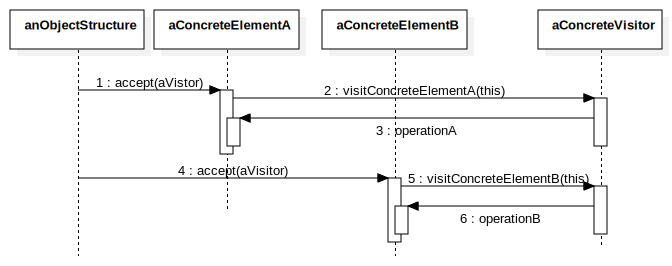
\includegraphics[width=\textwidth,height=\textheight,keepaspectratio]{images/visitor-pattern-sequence.pdf}
\caption{Sequence Diagram di un generico Visitor}
\label{fig:visitor-pattern-sequence}
\end{figure}

\subsection{Conseguenze}
Gli effetti che il Visitor ha su un progetto software sono molteplici:
\begin{enumerate}
\item Visitor consente di aggiungere facilmente operazioni a oggetti complessi. Infatti per definire una nuova operazione basterà definire un nuovo Visitor, senza quindi andare a modificare tutte le classi degli oggetti che compongono la struttura nel caso in cui questa operazione coinvolga più di uno di questi oggetti.
\item Aiuta a mantenere le operazioni correlate sotto la stessa classe e a separare quelle scorrelate.
\item Complica l'aggiunta di classi ConcreteElement, poiché questo implica l'aggiornamento di tutte le interfacce dei Visitor che devono poter visitare l'elemento. Quindi è auspicabile usare questo pattern nei casi in cui la struttura rimane invariata o comunque cambia con frequenza minore rispetto alle operazioni da eseguirvi.\\
Nei casi in cui la struttura di classi cambia frequentemente può diventare conveniente aggiungere le operazioni direttamente dentro queste classi.
\item Visitor al contrario di altri pattern come l'\textit{Iterator} non è vincolato a visitare oggetti appartenenti alla stessa classe.
\item Il funzionamento del Visitor è tale da imporre all'elemento concreto di implementare metodi pubblici che accedono al loro stato interno compromettendo quindi il loro incapsulamento.
\item Il Visitor ha il vantaggio di tenere traccia dell'attraversamento della struttura cosa che altrimenti deve essere passata tra i parametri dei vari metodi eseguiti sugli oggetti.
\end{enumerate}


 
